\chapter{Training Setup and Experiments}
\label{ch:experiments}

This chapter reports the training protocol and the four ablation
families that fix the operating point of the V5 JEPA system:
mask-policy mixture, EMA decay~$\tau$, mask ratio, and the scaling
step from sanity to thesis run. All evidence tags follow the rules
of Section~\ref{sec:arch-scale} (CONFIRMED, HYPOTHESIS, STALE).

\section{Protocol}
\label{sec:exp-protocol}

Training uses AdamW~\cite{loshchilov2019adamw} with a single
parameter group at learning rate $10^{-4}$ and weight decay
$5 \times 10^{-2}$, with cosine decay~\cite{loshchilov2017sgdr}
applied across the full epoch budget. Mixed-precision (\texttt{bf16}
autocast) and gradient checkpointing of the predictor are enabled on
both backends. The 5060\,Ti CUDA path uses
\texttt{torch.nn.functional.scaled\_dot\_product\_attention} directly;
the Apple~MPS path is routed through the manual sequence
$\mathrm{softmax}\!\bigl((QK^{\top})\,s\bigr)\,V$ with the mask
applied additively before the softmax, because the kernel returns
NaN under \texttt{torch.no\_grad} with a non-trivial
\texttt{attn\_mask} (Finding~F6). The two backends are not unified, because that would
silently break MPS evaluation.

A second numerical guardrail concerns the token-level pad mask. The
intersection $M_{\text{loss}} = M_{\text{mask}} \land M_{\text{valid}}
\land M_{\text{pad}}$ of Section~\ref{sec:arch-loss} is the only
correct denominator for the smooth-$L_{1}$ objective; an earlier
version that omitted $M_{\text{pad}}$ averaged gradients over padded
tokens and biased training toward the bucket boundary. The fix is in
\texttt{make\_token\_pad\_mask}; all results in this chapter use the
corrected denominator.

\section{Sanity history (E04--E09)}
\label{sec:exp-sanity}

Early sanity runs on four cubes established three results that
condition every later experiment. (1)~A mask-OFF baseline saturates
near epoch~24 (E06, best val~$0.0125$ at epoch~38), confirming that
the encoder memorises three training cubes when no occlusion is
applied (F4). (2)~A fast curriculum
($\mathit{tail\_only\_pct}{=}0.10$, $\mathit{warmup\_pct}{=}0.20$)
exhibits an eighteen-epoch plateau across epochs~7--31 of E05, with
best val~$0.0689$ at epoch~49 (F7). (3)~A slow curriculum
($0.25/0.40$) on the same configuration descends monotonically to
val~$0.00831$ at epoch~98 (E09), an eight-fold improvement over the
fast schedule (F1). The slow curriculum is the default everywhere
that follows.

Mask-ON and mask-OFF losses are not directly comparable: the former
averages only over masked target tokens (mask ratio~$\approx 0.8$),
while the latter averages over all tokens (F5). Comparisons in this
chapter are always within the mask-ON family.

\section{Mask-policy ablation (E12--E15)}
\label{sec:exp-mask}

Holding everything else fixed at the E09 anchor, four mask-policy
mixtures are compared on the four-cube sanity setup with the slow
curriculum. The best validation losses are summarised in
Table~\ref{tab:mask-policy} and the corresponding training curves in
Figure~\ref{fig:curves-mask}.

\begin{table}[htbp]
\centering
\begin{tabular}{lll}
\toprule
Run & Mixture $\{\text{tube},\text{future},\text{cross}\}$ & Best val \\
\midrule
E12 & $\{1.00, 0.00, 0.00\}$           & $0.04017$ (ep~42) \\
E13 & $\{0.70, 0.30, 0.00\}$           & $0.01812$ (ep~92) \\
E14 & $\{0.70, 0.00, 0.30\}$           & $0.01172$ (ep~91) \\
E15 & $\{0.34, 0.33, 0.33\}$           & $\mathbf{0.00530}$ (ep~99) \\
\bottomrule
\end{tabular}
\caption{Mask-policy ablation. All runs share the E09 anchor
(slow curriculum, $\tau{=}0.996$, ratio~$0.80$). The uniform mix is
$3.42\times$ better than tube-only and $1.57\times$ better than the
E09 tube-heavy default.}
\label{tab:mask-policy}
\end{table}

\begin{figure}[htbp]
\centering
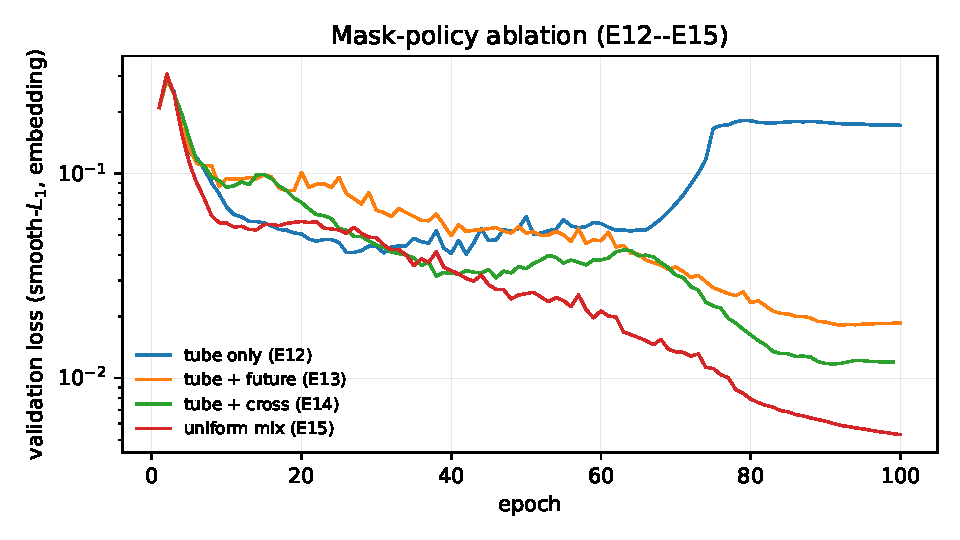
\includegraphics[width=0.92\linewidth]{assets/figures/curves_mask_policy.pdf}
\caption{Validation smooth-$L_{1}$ versus epoch for the four
mask-policy mixtures. E12 tube-only diverges after the
full-mix curriculum transition near epoch~65 while training loss
continues to fall, indicating policy under-coverage rather than
optimisation failure.}
\label{fig:curves-mask}
\end{figure}

Tube-only training (E12) diverges past the curriculum transition
on the single seed run: validation loss rises four-fold from
$0.040$ at epoch~42 to $0.172$ by epoch~99, while training loss
continues to decay (F3, HYPOTHESIS --- single-seed observation,
not reproduced across seeds). The interpretation, that future-block
and cross-time are load-bearing regularisers rather than
curriculum-pacing artefacts, is consistent with the divergence
post-curriculum and with the uniform-mix outperforming every
tube-heavy mixture, but is not established as a causal claim
from one run. Uniform weighting of the three policies is the new
sanity floor (F11) and is robust across the EMA and mask-ratio
sweeps that follow; E09's tube-heavy default over-weighted
tube-occlusion. All downstream sweeps are re-anchored on the
uniform mix.

\section{EMA decay sweep (E17--E20)}
\label{sec:exp-ema}

The target-encoder decay $\tau$ is swept across
$\{0.990, 0.994, 0.998, 0.9995\}$ at the E15 anchor.
Figure~\ref{fig:curves-ema} reports the validation curves and
Table~\ref{tab:ema-sweep} the best validation losses.

\begin{table}[htbp]
\centering
\begin{tabular}{lll}
\toprule
Run & $\tau$ & Best val \\
\midrule
E17 & $0.9900$ & $\mathbf{0.00761}$ \\
E18 & $0.9940$ & $0.00938$ \\
E19 & $0.9980$ & $0.01107$ \\
E20 & $0.9995$ & $0.03010$ \\
\bottomrule
\end{tabular}
\caption{EMA decay sweep at the uniform-mix anchor. The relation is
monotone: lower $\tau$ yields better validation, with $\tau{=}0.990$
the winner over the four-cube sanity scale.}
\label{tab:ema-sweep}
\end{table}

\begin{figure}[htbp]
\centering
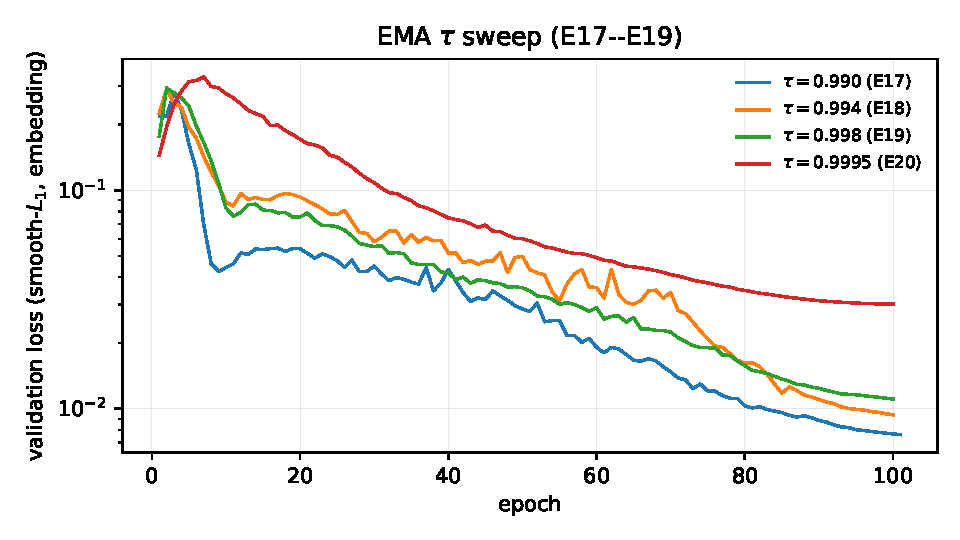
\includegraphics[width=0.92\linewidth]{assets/figures/curves_ema_sweep.pdf}
\caption{Validation smooth-$L_{1}$ versus epoch across four EMA
decay rates. The ordering $\tau{=}0.990 < 0.994 < 0.998 < 0.9995$
holds at every epoch past warmup.}
\label{fig:curves-ema}
\end{figure}

\section{Mask-ratio sweep (E25--E28)}
\label{sec:exp-ratio}

Holding the uniform mixture and $\tau{=}0.996$ fixed, the per-step
mask ratio is swept across $\{0.60, 0.75, 0.85, 0.90\}$. Among
the three runs trained to completion, $r{=}0.75$ (E26, val~$0.00876$)
is the winner over $r{=}0.60$ (E25, $0.00960$) and $r{=}0.85$
(E27, $0.01597$). The fourth arm, $r{=}0.90$ (E28), was terminated
at epoch~36 once its validation loss was worse than E27 at every
epoch logged, and the freed budget was redirected to the
thesis-scale run. The three completed arms are consistent with a
concave response peaked at the interior point, but the curve is
fitted on three points; the strict concavity claim is reported as
a winner-among-completed-arms result rather than as an established
maximum.

\section{Scaling to the thesis run (E29 -- E30)}
\label{sec:exp-scale}

Two failed attempts preceded the thesis-scale result. E29 launched
the full ViT-Small configuration with an 80-epoch budget across all
21 cubes; profiling at epoch~0 measured $4.9$~s/step and projected
an 11.5-day completion, which exceeded the available time budget,
and the run was killed after the first validation. E29b retried at
30\,000 optimiser steps, but plateaued at val~$0.0341$ near epoch~17
because the per-cube training budget of $\approx 1430$ steps was
insufficient to escape the tail-mask warmup regime.

E30 (the thesis run) reacts to both failure modes. Five cubes are
held out for the downstream probe; thirteen cubes train and three
validate. The optimiser budget is fixed at $100$ epochs of $2000$
steps each, $\approx 1.54 \times 10^{4}$ steps per training cube and
roughly three times the per-cube step count of the sanity scale.
Excluding the five largest cubes shrinks the bucketed batches that
limited throughput on E29b; measured throughput is $0.84$~s/step,
$5.8\times$ faster than E29b. The validation curve is shown in
Figure~\ref{fig:curves-thesis}.

\begin{figure}[htbp]
\centering
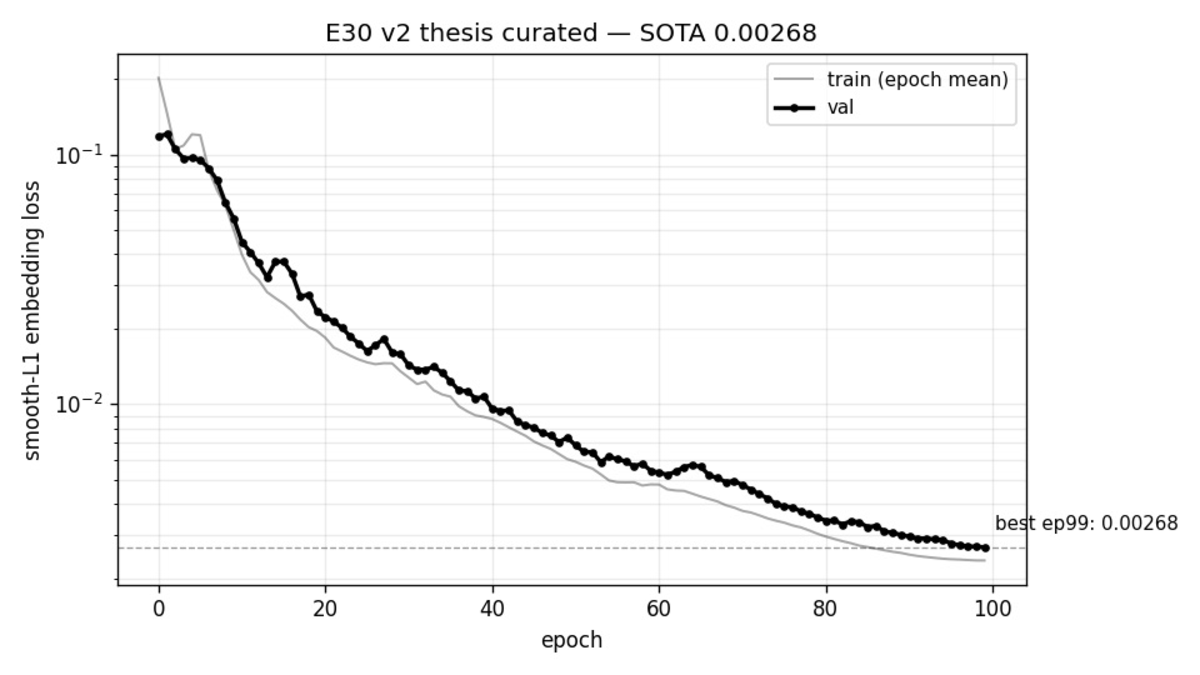
\includegraphics[width=0.78\linewidth]{assets/figures/curves_thesis_run.pdf}
\caption{Validation smooth-$L_{1}$ versus epoch for the E30 thesis
run (13 train / 3 val cubes, 100 epochs of 2000 steps each).}
\label{fig:curves-thesis}
\end{figure}

\section{Convergence summary}
\label{sec:exp-summary}

Figure~\ref{fig:ablation-summary} consolidates the best validation
loss recorded across the mask-policy, EMA, and mask-ratio sweeps as
well as the thesis run, with the corresponding numeric values
reproduced verbatim from the run logs in
Appendix~\ref{app:curves}.

\begin{figure}[htbp]
\centering
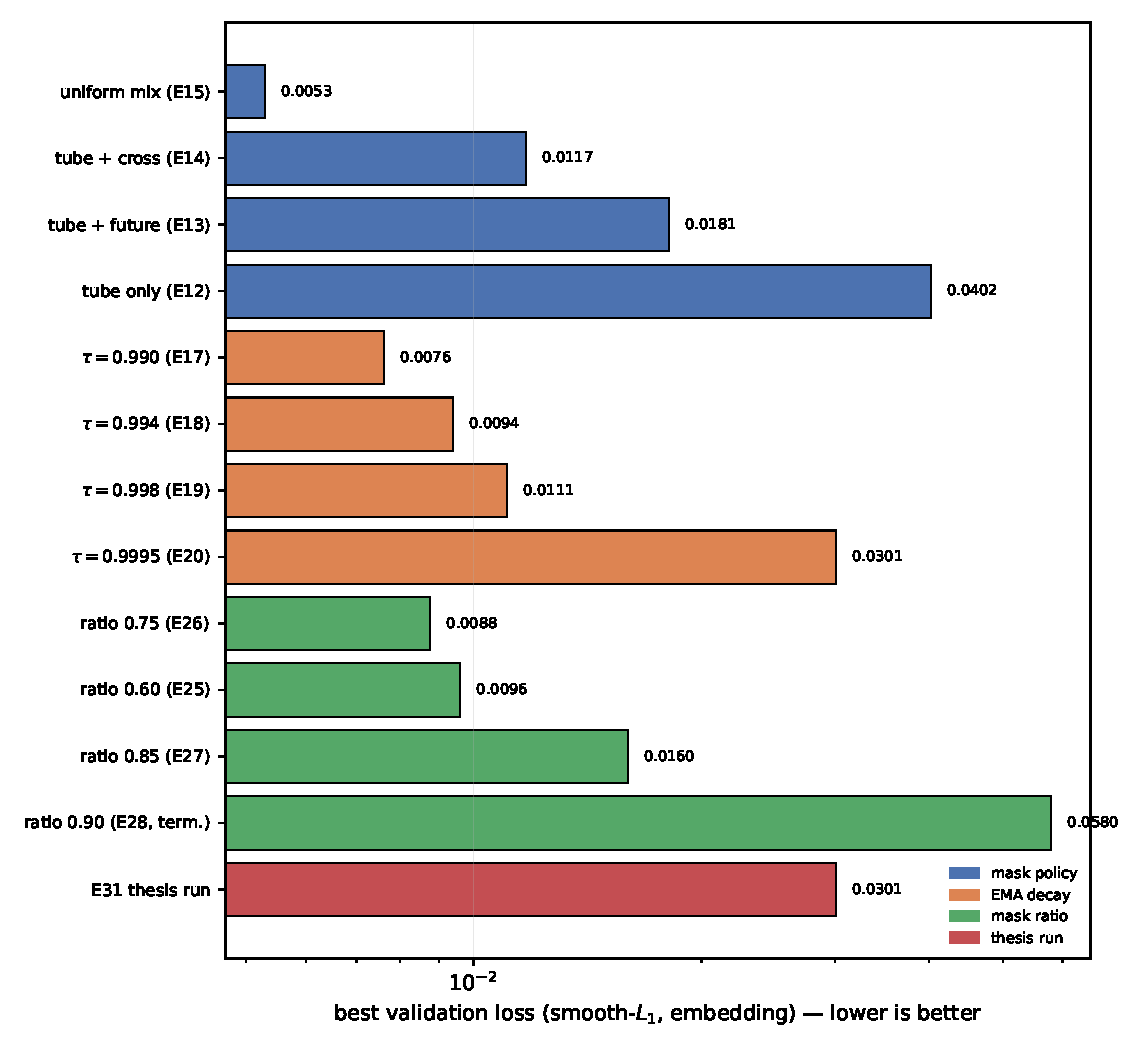
\includegraphics[width=0.92\linewidth]{assets/figures/ablation_summary.pdf}
\caption{Best validation loss across the four ablation families.
Lower is better; all sanity-scale arms share architecture, optimiser,
and curriculum, and differ only in the swept variable.}
\label{fig:ablation-summary}
\end{figure}

\section{Findings synthesis}
\label{sec:exp-findings}

Table~\ref{tab:findings} summarises the load-bearing findings that
condition the present work. Full statements and evidence are
recorded in the project log under the same labels.

\begin{table}[htbp]
\centering
\small
\begin{tabular}{p{0.08\linewidth}p{0.78\linewidth}p{0.10\linewidth}}
\toprule
ID & Statement & Tag \\
\midrule
F1  & Slow curriculum ($0.25/0.40$) is the default; $8\times$ better than fast at sanity scale. & CONFIRMED \\
F2  & $|W| \leq 10^{8}$ guard preserves the legitimate $10^{5}$--$10^{7}$ peaks; $10^{5}$ guard destroys signal. & CONFIRMED \\
F3  & Tube-only masking diverges past curriculum transition on the single seed observed; future and cross-time are interpreted as load-bearing regularisers. & HYPOTHESIS \\
F4  & Mask-OFF saturates at sanity scale near epoch~24; informative only as early baseline. & CONFIRMED \\
F5  & Mask-ON and mask-OFF losses are not directly comparable (different denominators). & CONFIRMED \\
F6  & MPS \texttt{SDPA} returns NaN under \texttt{no\_grad} with \texttt{attn\_mask}; manual path required. & CONFIRMED \\
F7  & Fast curriculum induces an 18-epoch plateau; superseded by F1. & CONFIRMED \\
F8  & Sanity floor at uniform mix is val~$0.00530$ (E15). & CONFIRMED \\
F9  & Frozen E30~v2 features carry phase, temporal, and (post per-cube log-affine fit) absolute-scale structure on novel cubes; four of five novel cubes beat lag-one persistence after one $(a, b)$ fit. & CONFIRMED \\
F10 & Path~A (LoRA on Surya) abandoned: architectural lock on $4096 / 60$-min $/ 13$-channel inputs. & CONFIRMED \\
F11 & Uniform mask mixture dominates every tube-heavy variant tested. & CONFIRMED \\
F12 & Cross-attention predictor must drop causal masking in the masked pretext path. & CONFIRMED \\
F13 & C$+$/12~h MLP head beats lag-one persistence on harp\_49 (AUC $= 1.000$ vs $0.975$); does not transfer uniformly across the eight mixed-label evaluation cubes. & CONFIRMED \\
\bottomrule
\end{tabular}
\caption{Findings carried forward into the downstream probe of
Chapter~\ref{ch:probe} and the future work of
Chapter~\ref{ch:summary}.}
\label{tab:findings}
\end{table}

